\chapter{Design}

\section{Overall System Design}

\subsection{Short description of the main parts of the system}

Hardware Allocation Database

\begin{itemize}
\item IT staff user interface
\item Line manager user inferface
\item Staff user interface
\item Login screen
\item Viewing Databases
\item Editing Databases
\end{itemize}

\

\textbf{IT staff user interface}

\begin{itemize}
\item IT staff have admin rights to the system. They will be able to view everyones information and are the only people who may edit information on the system.
\item Once logged in they will be presented with a user interface with buttons allowing them to open a database or search for staff.
\item All IT staff will share a username and password.
\item The search function will take the user to an interface which will allow them to search for a staff member and be shown which hardware devices they own. This search could also be performed by going to the staff database and using the search function there, but this may be used frequently and so is placed here for convience.
\item The open database button will take them to a user interface that will have a dropdown box allowing them to pick which database to view. There will also be a "Continue" button to click when the database is selected and the database will be presented to them. There will also be a "Edit Database" button to edit, add or remove entries. A search button will also be on this screen to allow the user to search for a specific field.
\item The edit database will allow the user to change information on the database.
\end{itemize}

\

\textbf{Line manager user interface}

\begin{itemize}
\item Line manager's have more rights than normal staff but unlike IT staff they cannot edit any information.
\item Line manager's share the same username if they are part of the same department (for example someone from Liverpool Financing will use the same username as someone from Orwell Financing) and a password that they may change at any time. Upon first using the system their password will be issued by IT staff. Their username will be a 5 digit number allocated to them by IT staff (the best way to do this will be via email). 
\item Line manager's can view information of members from their own department.
\item Once logged in, the user interface will show a "View Department" button and a "View My Information" button.
\item The "View Department" button will show the staff database but only show records from staff at their own department. There will be a search function to find a specific field.
\item The "View My Information" button will allow the user to view their own hardware devices and personal information. It may be used often to check the warranty period of an item and to check correct information is being displayed.
\end{itemize}

\

\textbf{Staff User Interface}
\begin{itemize}
\item Ordinary staff members will all have unique usernames and be able to create their own password.
\item After logging on they will be taken to a user interface with a button called "View My Information".
\item The "View My Information" button will allow the user to view their own hardware devices and personal information. It may be used often to check the warranty period of an item and to check correct information is being displayed.
\end{itemize}

\

\textbf{Login screen}
\begin{itemize}
\item The login screen will have a username field and a password field. There will also be two buttons, one to login and the other will be "Forgot Your Password?".
\item The "Forgot Your Password?" button will take the user to another interface which will ask for their Volac (company) email address, Forename and Surname. This information will be sent to the IT staff who can review it and email the user another password to use or tell them what their password was. It is important to note that all Volac staff have the same buisness email (for example XXX.Volac.com), this means SMTP settings can be set up easily in Python. This process will be easier than asking IT Staff directly.
\item Normal staff all have their own username and a password that they may change at any time. Upon first using the system their password will be issued by IT staff. Their username will be a 5 digit number allocated to them by IT staff (the best way to do this will be via email). 
\item Line manager's share the same username if they are part of the same department (for example someone from Liverpool Financing will use the same username as someone from Orwell Financing) and a password that they may change at any time. Upon first using the system their password will be issued by IT staff. Their username will be a 5 digit number allocated to them by IT staff (the best way to do this will be via email). 
\item All IT staff will share a username and password to have admin rights.
\item There are 100,000 combinations on a 5 digit number (10$^5$) which will be more than enough for the company, it will be best to start from the left and issue 10000 to IT staff and start with 20000 for other staff (and proceed with 20001, 20002, ... 20010...)
\end{itemize}

\

\textbf{Viewing Databases}

\begin{itemize}
\item All staff, in some way, will be able to view a database.
\item For general staff, they will only be able to view their own data. Line Manager's will be able to view all data in the staff database about the members in their department. IT staff have full access to all databases to view all information.
\item A dropdown box will be useful for IT staff to pick a database to view, buttons will surffice for other staff since they can only view a couple of databases.
\end{itemize}

\

\textbf{Editing Databases}
\begin{itemize}
\item To add entries the user will click the "Edit Database" button (found on the IT staff interface).
\item This button will then allow the user to either edit existing data or take the user to a form which allows data to be input into fields for such things as First Name, Surname, Warranty or Hardware Device.
\item Validation will be required for various fields such as telephone numbers (string of length 11) and dropdown boxes will be used for boolean values for fields such as Warranty.
\end{itemize}


\subsection{System flowcharts showing an overview of the complete system}

\begin{figure}[H]
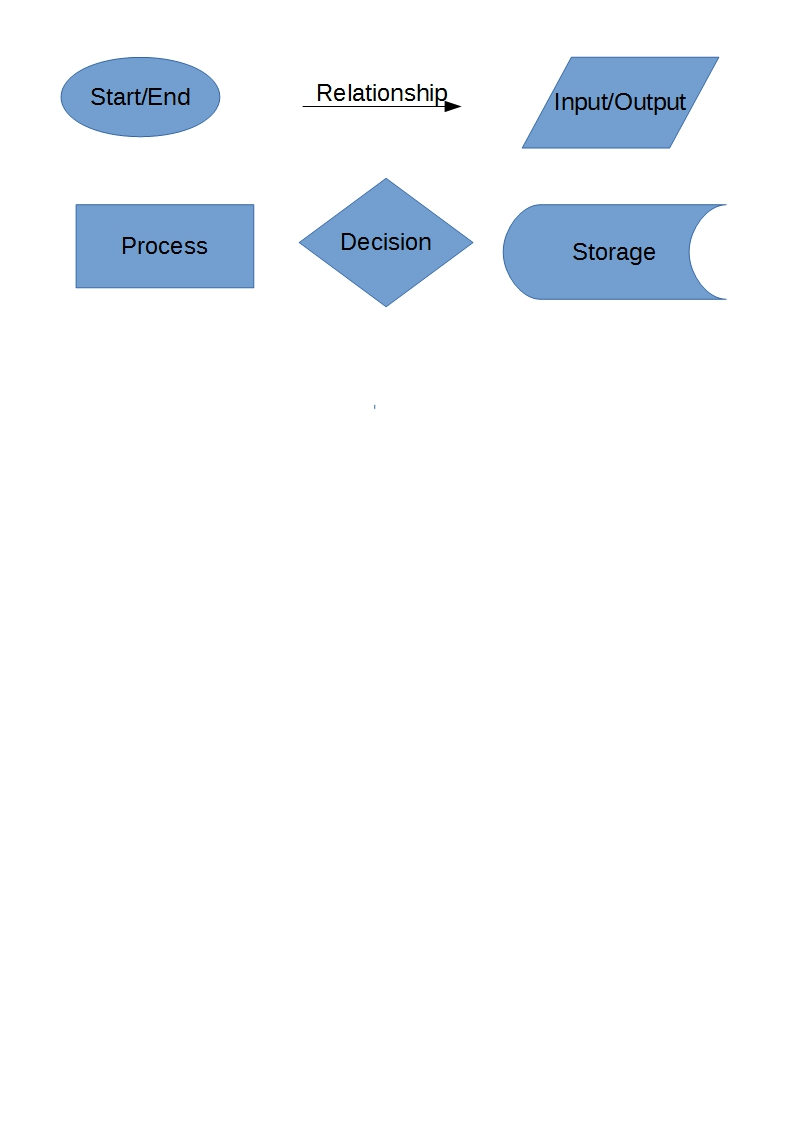
\includegraphics[width=.9\textwidth,height=.9\textheight,keepaspectratio]{FlowchartKey.jpg}
\end{figure}

\newpage

\begin{figure}[H]
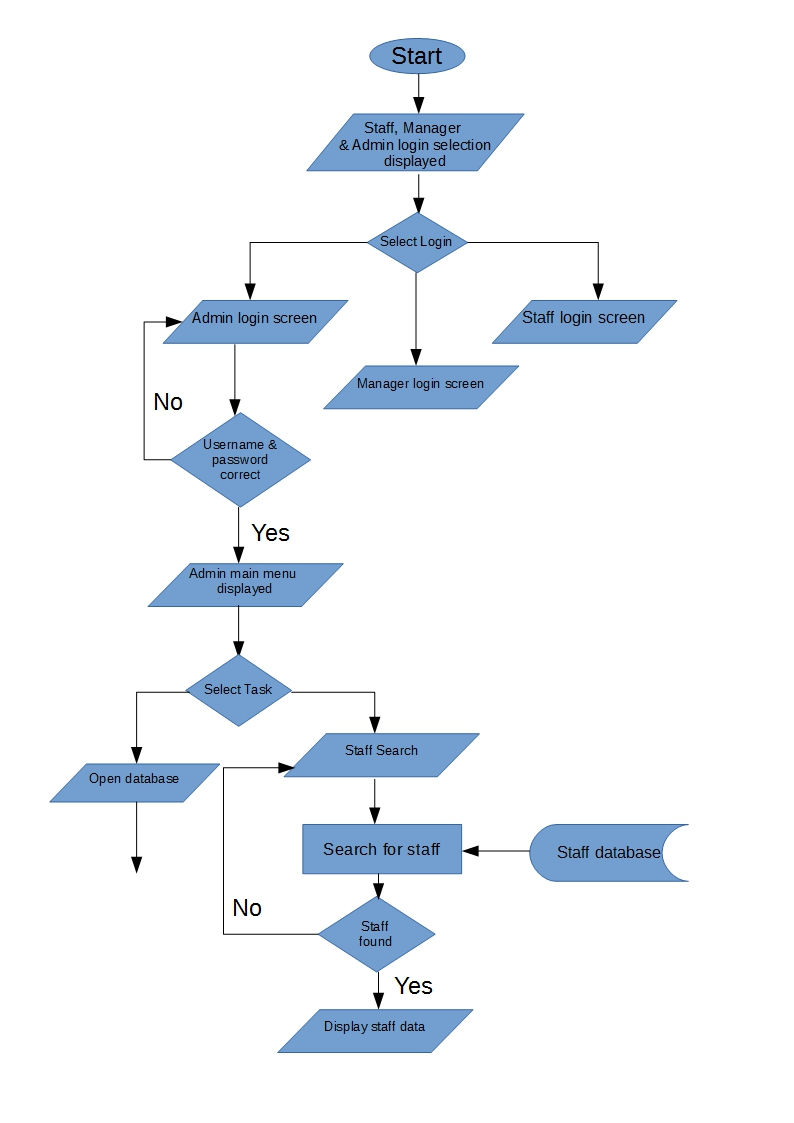
\includegraphics[width=\textwidth]{FlowchartPart1.jpg}
\end{figure}

\begin{figure}[H]
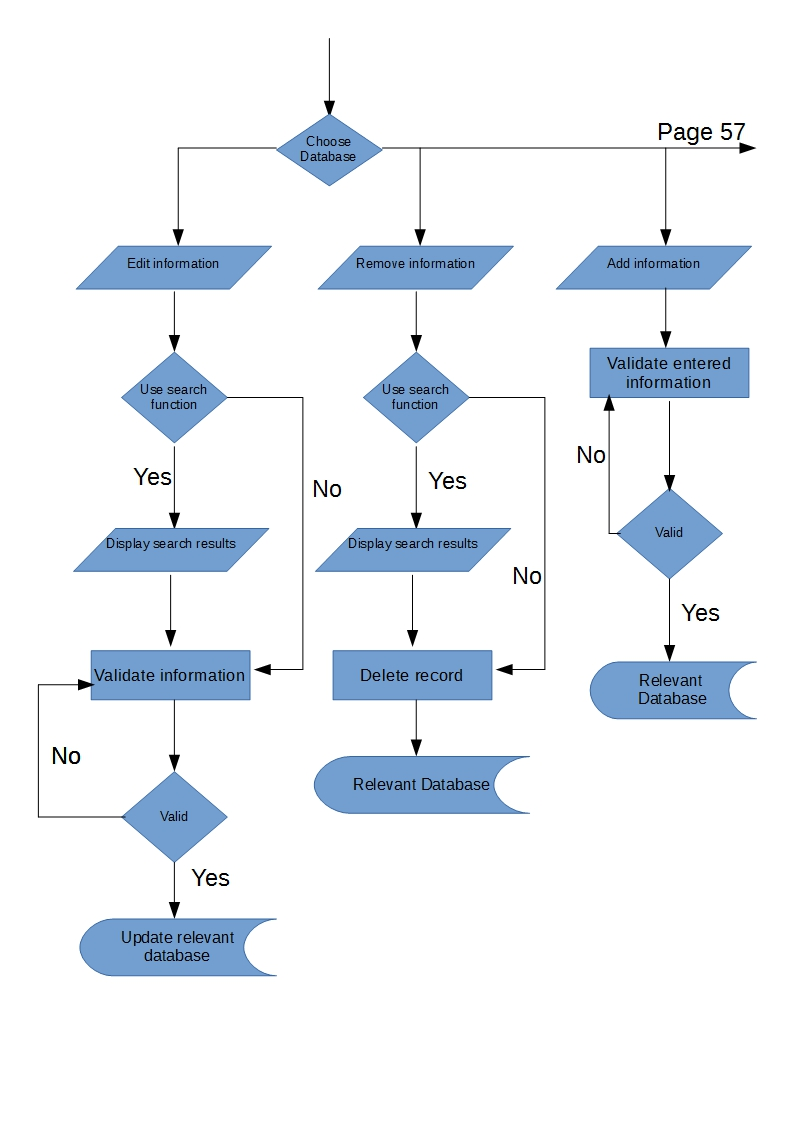
\includegraphics[width=\textwidth]{FlowchartPart2.jpg}
\end{figure}

\begin{figure}[H]
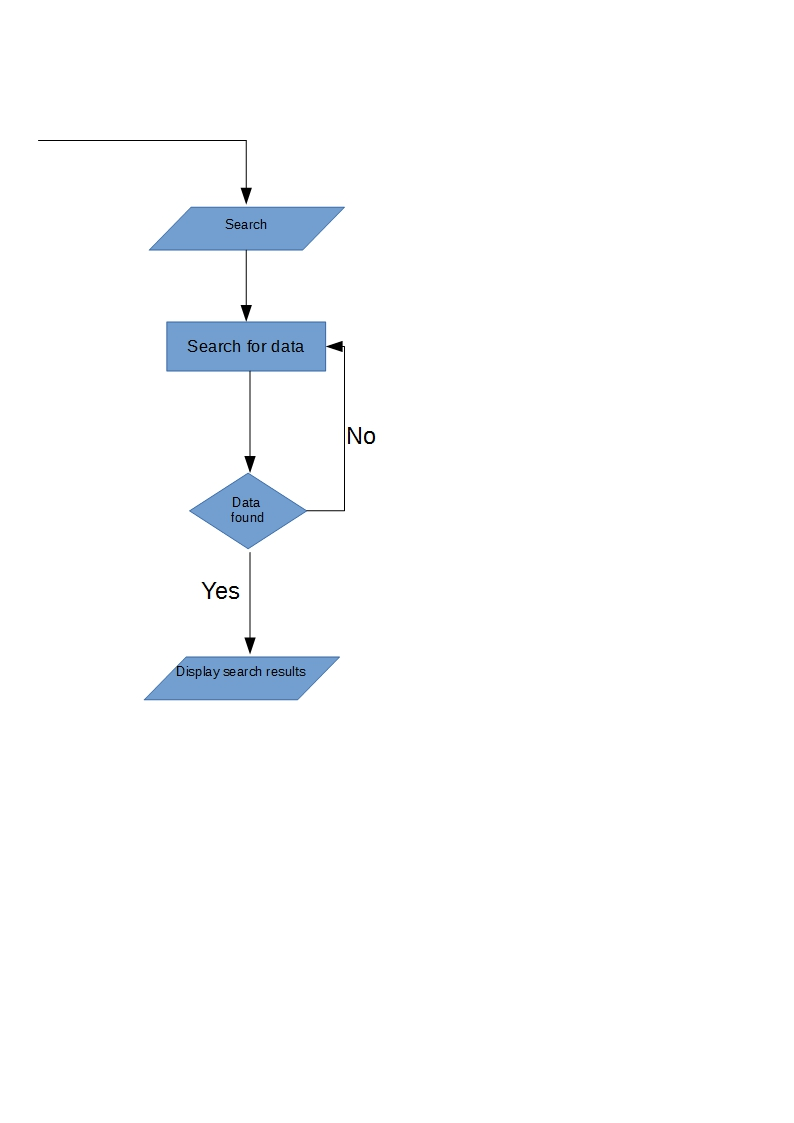
\includegraphics[width=\textwidth]{FlowchartPart3.jpg}
\end{figure}

\begin{figure}[H]
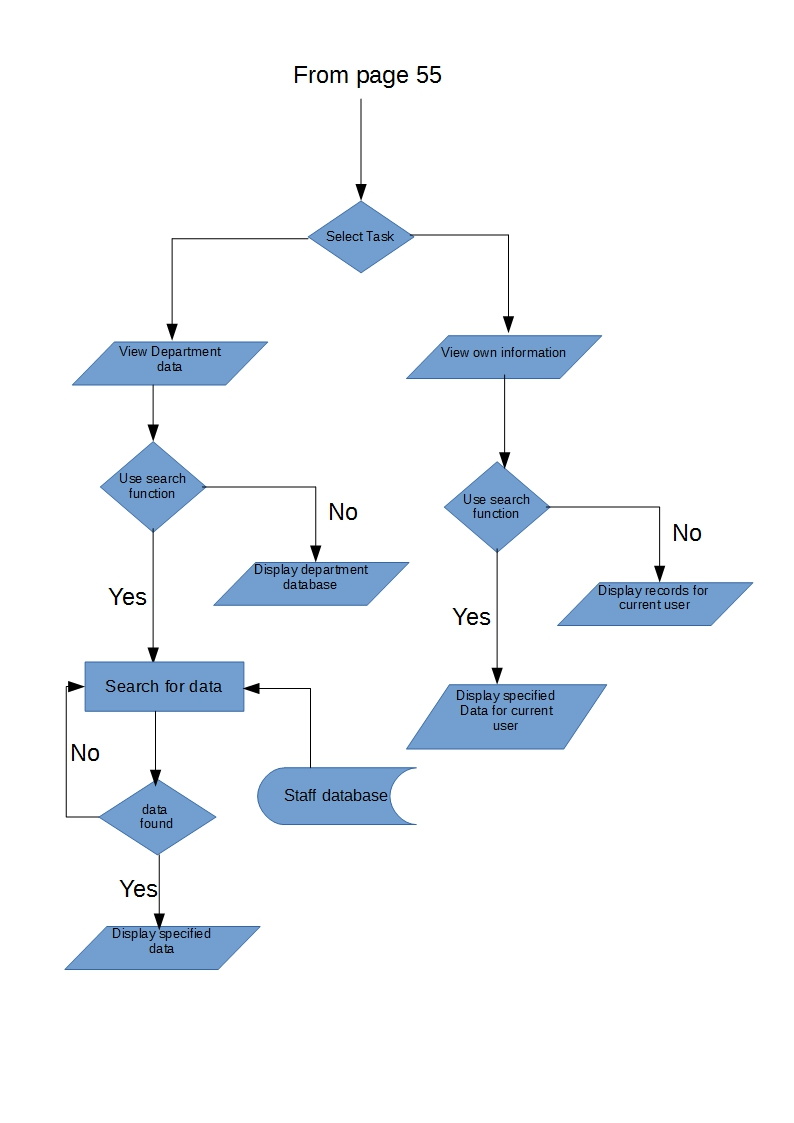
\includegraphics[width=\textwidth]{FlowchartPart4.jpg}
\end{figure}

\begin{figure}[H]
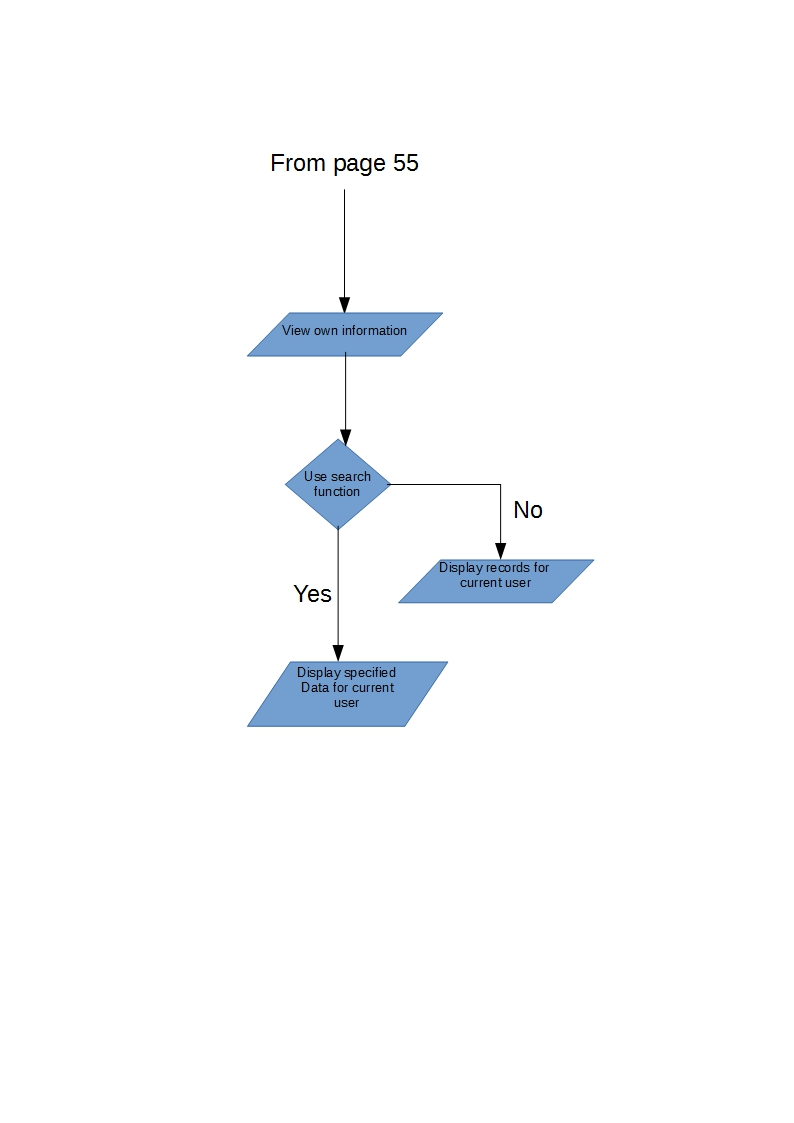
\includegraphics[width=\textwidth]{FlowchartPart5.jpg}
\end{figure}



\section{User Interface Designs}

\section{Program Structure}

\section {Hardware Specification}

The system will be stored onto a server stored in the workplace which is perfectly capable to handle the system, the specs are as followed:
\begin{itemize}
\item HP DL360
\item Windows 2003 (can run any operating system required)
\item 4TB Hard Drive
\item 16GB RAM
\item Quad Core Processor - 2.5 GHZ
\end{itemize}
The server is stored in a server room with high ventilation and fans operated 24/7. This is a huge benefit because the system can be running at all times so people can access the database. Preferably the overall model will be client-server and each user will have their own login for security. All users should connect using clients on local computers and will not directly access the server.

Users will connect to the system using their own computers at the workplace. These computers all have Windows 7 installed and run at the resolution of 1920x1080. The monitor sizes range from different locations, but the smallest would be 21" LCD monitors and the largest would be 27". These sizes will not be a problem since the application can fit on these monitors. All computers have a mouse, which is required for clicking the interface buttons, and a keyboard which is required for entering information. This system will not be developed for touch screen devices. The data for the program will be held on a hard drive inside the server that can be accessed by everyone who is connected to it. The company will not need any additional hardware to run the proposed system.

\subsection{Top-down design structure charts}

\subsection{Algorithms in pseudo-code for each data transformation process}

\subsection{Object Diagrams}

\subsection{Class Definitions}

\section{Prototyping}

\section{Definition of Data Requirements}

\subsection{Identification of all data input items}

\subsection{Identification of all data output items}

\subsection{Explanation of how data output items are generated}

\subsection{Data Dictionary}

\subsection{Identification of appropriate storage media}

\section{Database Design}

\subsection{Normalisation}

\newpage

\subsubsection{ER Diagrams}

\begin{figure}[H]
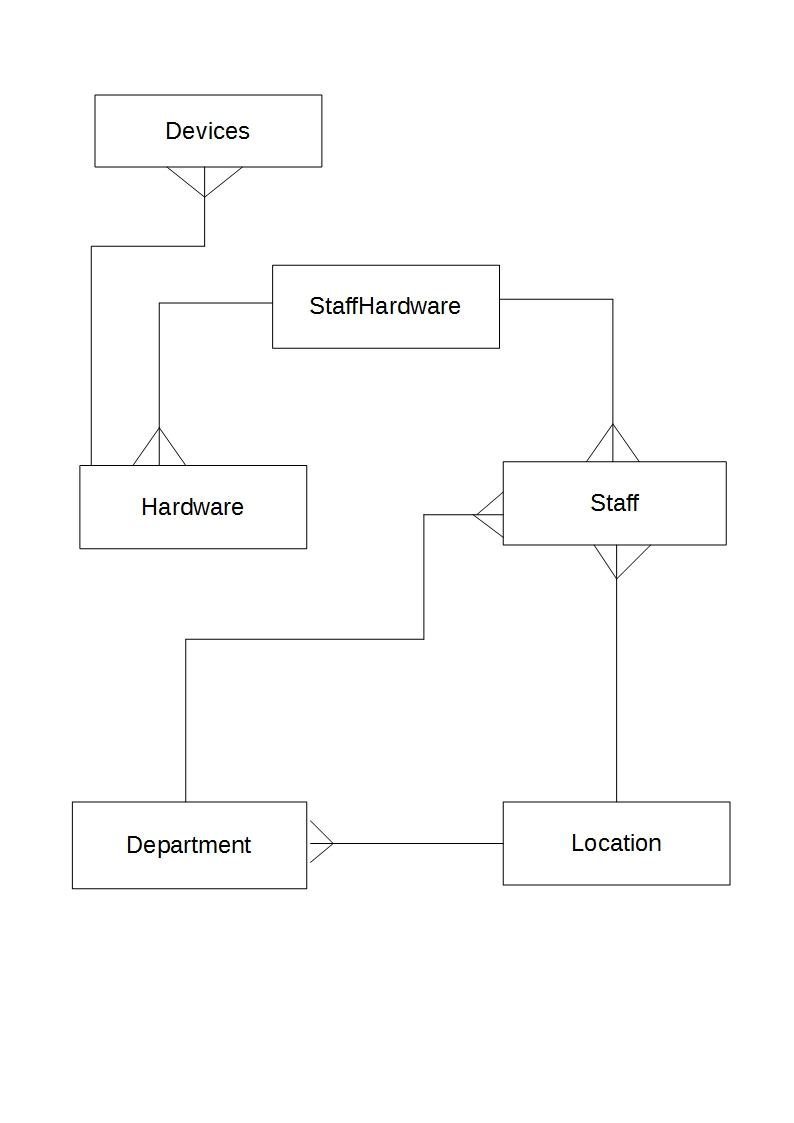
\includegraphics[width=\textwidth]{ERNormalisedDiagram.jpg}
\end{figure}


\subsubsection{Entity Descriptions}


\textbf{Staff}  (\underline{StaffID}, FirstName, LastName, JobTitle, \textit{DepartmentID},\\ \textit{ LocationID})


\

\textbf{Hardware}  (\underline{HardwareID}, \textit{DeviceID},  \textit{HardwareModelID},\\ HardwareCost, HardwareWarranty, HardwareWarrantyPeriod,\\ HardwareSerialNumber, 		HardwareIMEINumber, \\HardwarePhoneNumber)

\

\textbf{HardwareMake} (\underline{HardwareMakeID}, HardwareMakeName)

\

\textbf{HardwareModel} (\underline{HardwareModelID}, HardwareModelName, \textit{HardwareMakeID})

\


\textbf{DeviceType}  (\underline{DeviceID}, DeviceName)


\


\textbf{StaffHardware}  (\underline{ StaffID}, \underline{ HardwareID},PurchaseDate)


\


\textbf{Department}  (\underline{DepartmentID}, DepartmentName)


\


\textbf{Location}  (\underline{LocationID}, LocationName, LocationAddrLine1, LocationAddrLine2, LocationAddrLine3)

\

\textbf{DepartmentLocation} (\underline{LocationID}, \underline{DepartmentID})




\subsubsection{1NF to 3NF}

\begin{figure}[H]
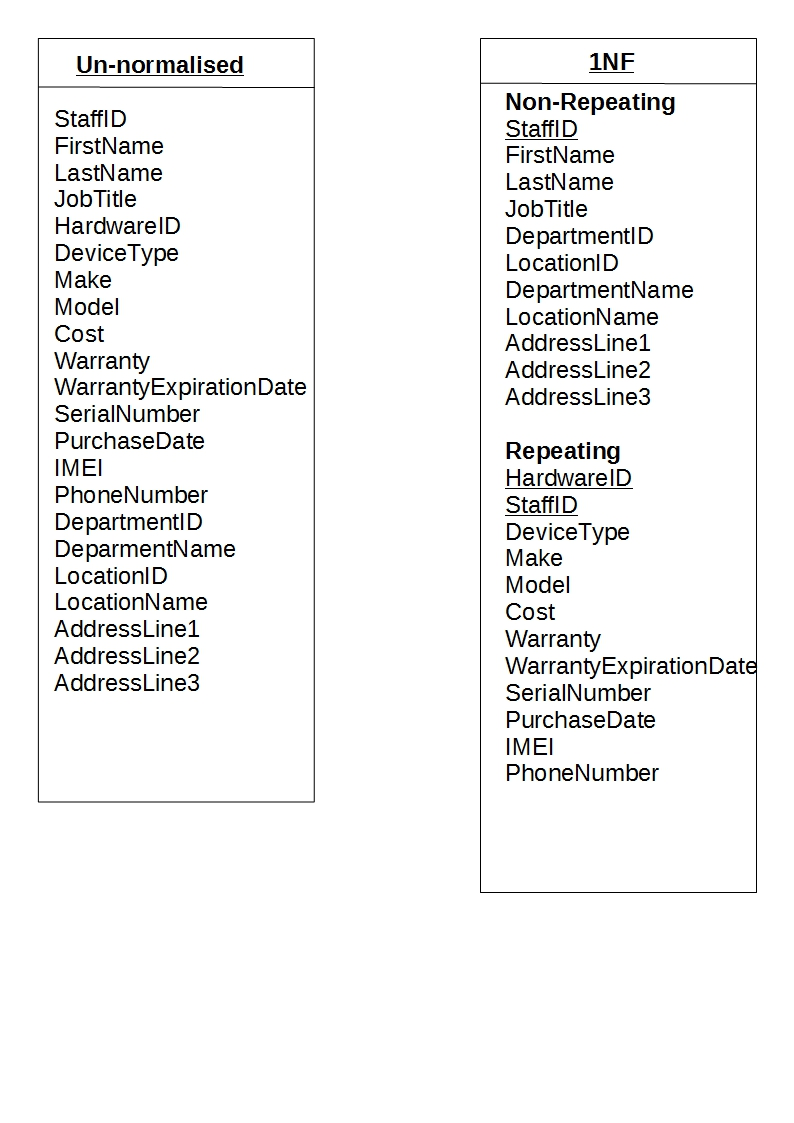
\includegraphics[width=\textwidth]{UNF&1NF.jpg}
\end{figure}

\begin{figure}[H]
\includegraphics[width=\textwidth]{2NF.jpg}
\end{figure}

\begin{figure}[H]
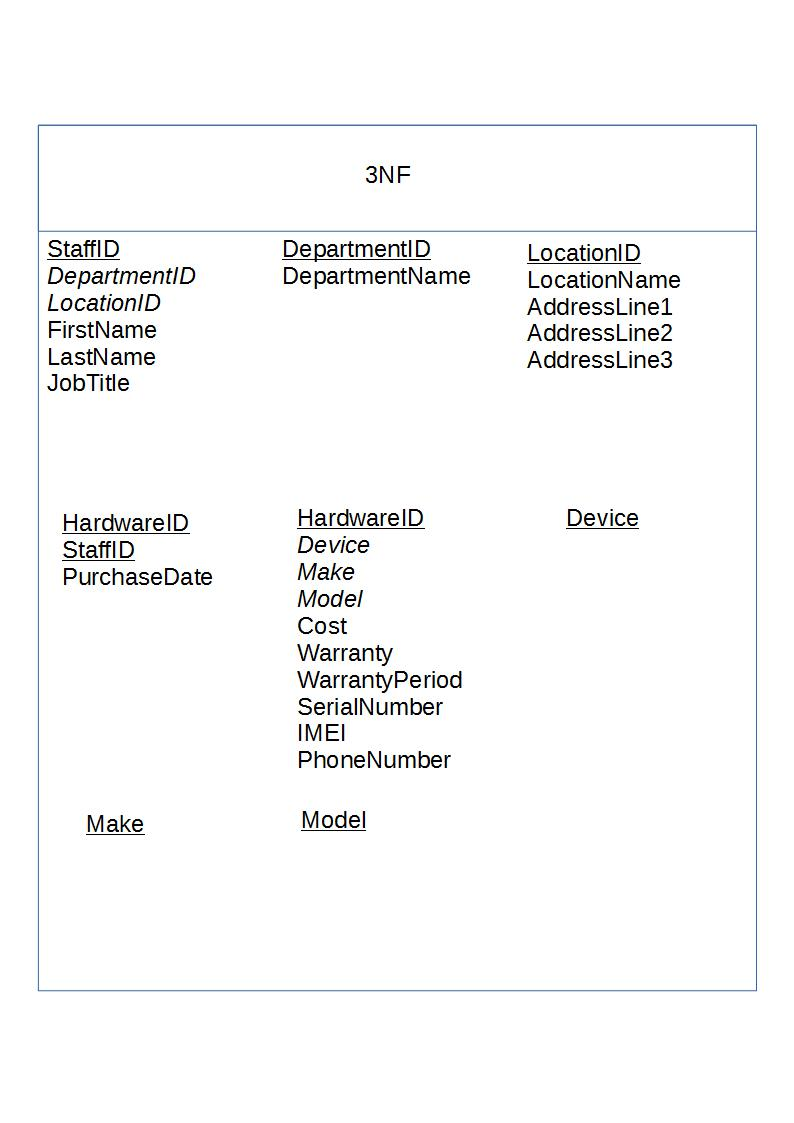
\includegraphics[width=\textwidth]{3NF.jpg}
\end{figure}

\begin{center}
\begin{tabular}{|p{6cm}|p{5cm}|}
\hline
\textbf{SQL}      & \textbf{Description} \\ \hline
"""create table Staff(\

   StaffID INTEGER,\

   FirstName TEXT,\

   LastName TEXT,\

   JobTitle TEXT,\

   DepartmentID INTEGER,\

   LocationID INTEGER,\

   PRIMARY KEY(StaffID))\

   FOREIGN KEY(DepartmentID) \

   REFERENCES Department(DepartmentID)\

   FOREIGN KEY(LocationID) \

   REFERENCES Location(LocationID)) """                         & This SQL statement will create a new table called Staff with the attributes - StaffID, FirstName, LastName, JobTitle, DepartmentID, LocationID, The primary key is StaffID and the foreign keys are DepartmentID and LocationID                       \\ \hline

"""insert into\

Staff(FirstName,LastName, JobTitle, DepartmentID) values
(‘{0}’,’{1}’,’{2}’,'{3}')
""".format(FirstName, LastName, JobTitle, DepartmentID) & This SQL statement will add 3 new records to the database. In this example it is eneterng a new staff record with attributes: FirstName, LastName, JobTitle and DepartmentID \\ \hline

"""delete from Staff\

where StaffID = ‘{3}’\

""".format(StaffID) & This statement will delete the staff member from the Staff table with the StaffID of {3} \\ \hline

\end{tabular}
\end{center}

\section{Security and Integrity of the System and Data}

\subsection{Security and Integrity of Data}

\subsection{System Security}

\section{Validation}

\section{Testing}

\begin{landscape}
\subsection{Outline Plan}

\begin{center}
    \begin{tabular}{|p{2cm}|p{5cm}|p{5cm}|p{4cm}|}
        \hline
        \textbf{Test Series} & \textbf{Purpose of Test Series} & \textbf{Testing Strategy} & \textbf{Strategy Rationale}\\ \hline
        Example & Example & Example & Example \\ \hline
    \end{tabular}
\end{center}

\subsection{Detailed Plan}

\begin{center}
    \begin{longtable}{|p{1.5cm}|p{2.5cm}|p{2.5cm}|p{2cm}|p{2cm}|p{2cm}|p{2cm}|p{2cm}|}
        \hline
        \textbf{Test Series} & \textbf{Purpose of Test} & \textbf{Test Description} & \textbf{Test Data} & \textbf{Test Data Type (Normal/ Erroneous/ Boundary)} & \textbf{Expected Result} & \textbf{Actual Result} & \textbf{Evidence}\\ \hline
        Example & Example & Example & Example & Example & Example & Example & Example \\ \hline
    \end{longtable}
\end{center}
\end{landscape}
